%%%%%%%%%%%%%%%%%%%%%%%%%%%%%%%%%%%%%%%%%%%%%%%%%%%%%%%%%%%
%%%%%%%%%%%%%%%%%%%%%%%%%%%%%%%%%%%%%%%%%%%%%%%%%%%%%%%%%%%
\subsection{EMMA}
\label{sec:res-emma}
%%%%%%%%%%%%%%%%%%%%%%%%%%%%%%%%%%%%%%%%%%%%%%%%%%%%%%%%%%%%%%%%%%%%%%%%%%%%%%%%%%%%%%%%5
%%% ALL SAMPLES
A total of 30 recipes (see appendix \ref{sec:app-emma}) have been investigated in 
five iterations ($t = 0, \dots, 4$) of the algorithm. 
Where the first generation encompassed 10 particles and each subsequent generation encompassed 5 particles. 
The best recipes for each generation can be seen in table \ref{tab:emma-Gb}. 
The experiments for generation 5 where not executed but 
predictions were already made
with the information from the previous generations. 
%%% BEST PREDICTED RECIPE
The best sample predicted by the algorithm is experiment number 13 with 
%lowest solution concentration, second highest layer count, lowest \gls{db} velocity and temperature, 
%and lowest calcination heating rate and temperature. 
lowest $c_{zr}$, $v_{DB}$, $T_{DB}$, $v_{cal}$, $T_{cal}$ and second highest $\lambda$. 
%lowest solution concentration, second highest layer count, lowest \gls{db} velocity and temperature, 
%and lowest calcination heating rate and temperature. 

\begin{table}[htb]
	\centering
    \caption{Global best per generation}
	\label{tab:emma-Gb}
	\begin{tabular}{ccccccccc}
        \hline\hline
		generation& measurements &enr &$c_{zr}$ &$\lambda$ &$v_{DB}$ &$T_{DB}$ &$v_{cal}$ &$T_{cal}$\\
        \hline
	1  &10	&1       &2    &4   &10   &40  &120  &300\\
	2  &15	&5       &2    &6   &10   &40  &120  &300\\
	3  &20	&2947    &4    &6   &16   &80 &1080  &300\\
	4  &25	&2405    &2    &6   &10   &40 &1080  &300\\
	5  &30	&13      &2   &10   &10   &40  &120  &300\\
    \hline\hline
	\end{tabular}
\end{table}

\begin{table}
	\centering
    \caption{Predicted $\hat{\gamma}$} 
    \label{tab:emma-pred-G}
    \begin{tabular}{cccccc}
        \hline\hline
    enr &1st gen \gls{rf}   &2nd gen \gls{rf} &3rd gen \gls{rf}    &4th gen \gls{rf}   &5th gen \gls{rf}\\
        \hline
    1       &1.214185    &       &       &       &38.7962       \\
    5       &       &4.196626       &       &       &25.47335       \\
    2947    &       &       &10.9594    &       &10.9594       \\
    2405    &       &       &       &20.04962   &25.47335       \\
    13      &       &       &       &       &24.87178   \\
        \hline\hline
    \end{tabular}
\end{table}

%%% OVER TIME 
The only clear trend from table \ref{tab:emma-Gb} is the layer count, which rises with the generations. 
The remaining input variables remained more or less the same except for the 3rd generation. 
\td{why?}
%
In table \ref{tab:emma-pred-G} it can be seen that the predicted $\hat{\gamma}$ 
(predicted with 5th generation \gls{rf}; see last column) lowered with each iteration, 
except for sample 2947, which wasn't predicted but measured. 
This shows that the easiest part of the algorithm - the selection of the optimum 
from predicted values - works as expected. 
% and that the predictions included more lower values over time
%
Contrarily, the predicted $\hat{\gamma}$ for each generation's best 
(predicted by the very generation's \gls{rf}) does increase with each iteration 
(see diagonal in table~\ref{tab:emma-pred-G}). 
This indicates an underestimation of $\hat\gamma$ at the beginning and a correction with time. 
%The reason for is probably a 
The underestimation probably stems from a lucky selection of initial experiments or a skew in the measurements. 
Indeed, the samples with the lowest \textit{optimisands} are amoung the first generation (see figure \ref{fig:emma-G-gen}, figure \ref{fig:emma-phd-gen} and appendix \ref{sec:app-emma}).

In figure \ref{fig:emma-gen} we can see the two measured main \textit{optimisands}, 
$\gamma$ and $\rho$, of each particle at generations 1 to 4. 
%for each particle included in the optimization. 
%It shows a clear trend which indicates that the optimization worked even though 
Both variables were to be minimized and show a clear trend towards low values with increasing generation, 
indicating that the optimization worked even though 
the prediction functions (see equations (\ref{eq:emma-phd3}) - (\ref{eq:emma-vcal4})) 
and the chosen samples where not exactly as expected. 
Neither were the measurements for these samples, which might be due to the high measuring error of samples and variation of quality due to uncontrolled independent variables like room temperature or humidity. 

\begin{figure}[hb]
    \centering
    \begin{subfigure}{.24\textwidth}
        \centering
        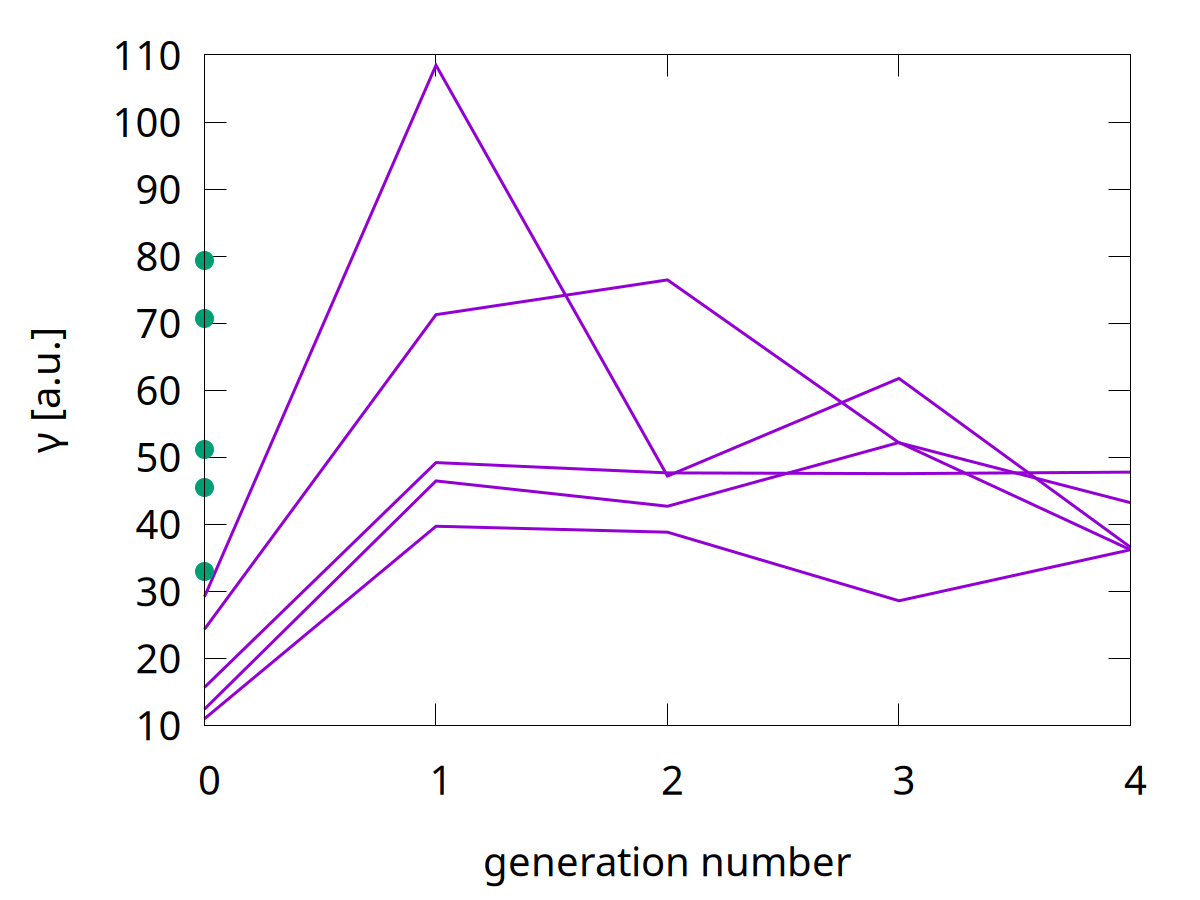
\includegraphics[width=.98\textwidth]{Pics/stats/gen-G.png}
        \caption{} \label{fig:emma-G-gen}
    \end{subfigure}
    \begin{subfigure}{.24\textwidth}
        \centering
        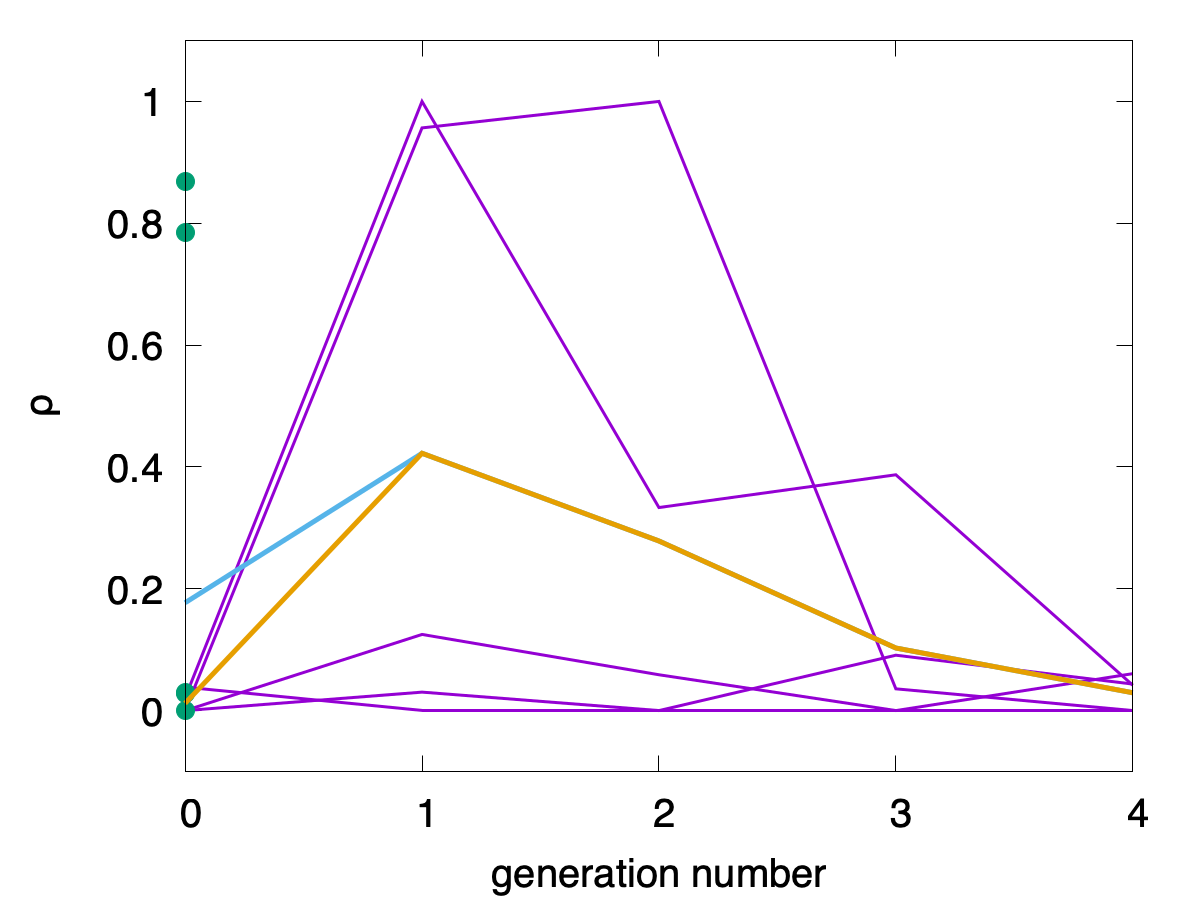
\includegraphics[width=.98\textwidth]{Pics/stats/gen-phd.png}
        \caption{} \label{fig:emma-phd-gen}
    \end{subfigure}
    \begin{subfigure}{.24\textwidth}
        \centering
        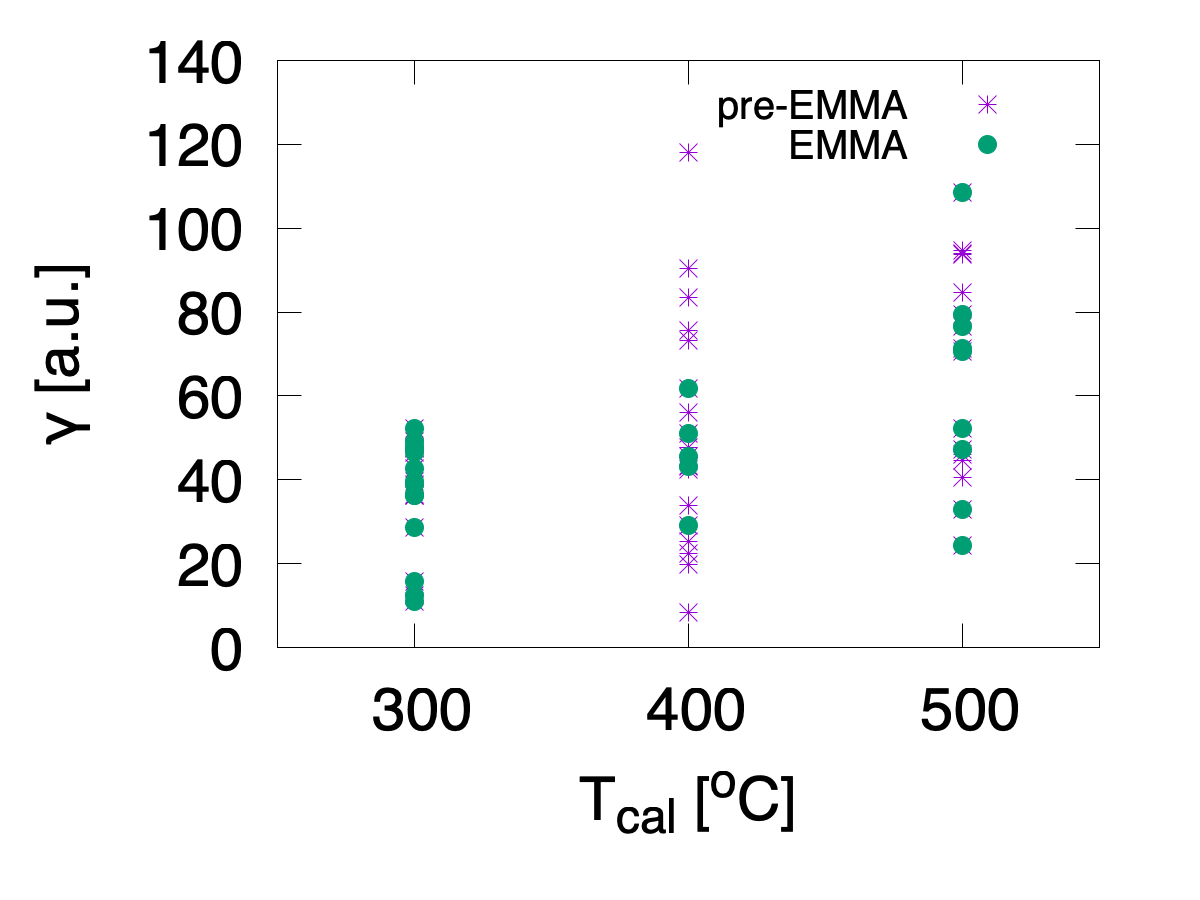
\includegraphics[width=.98\textwidth]{Pics/stats/G-tcal.png}
        \caption{} \label{fig:g-tcal}
    \end{subfigure}
    \begin{subfigure}{.24\textwidth}
        \centering
        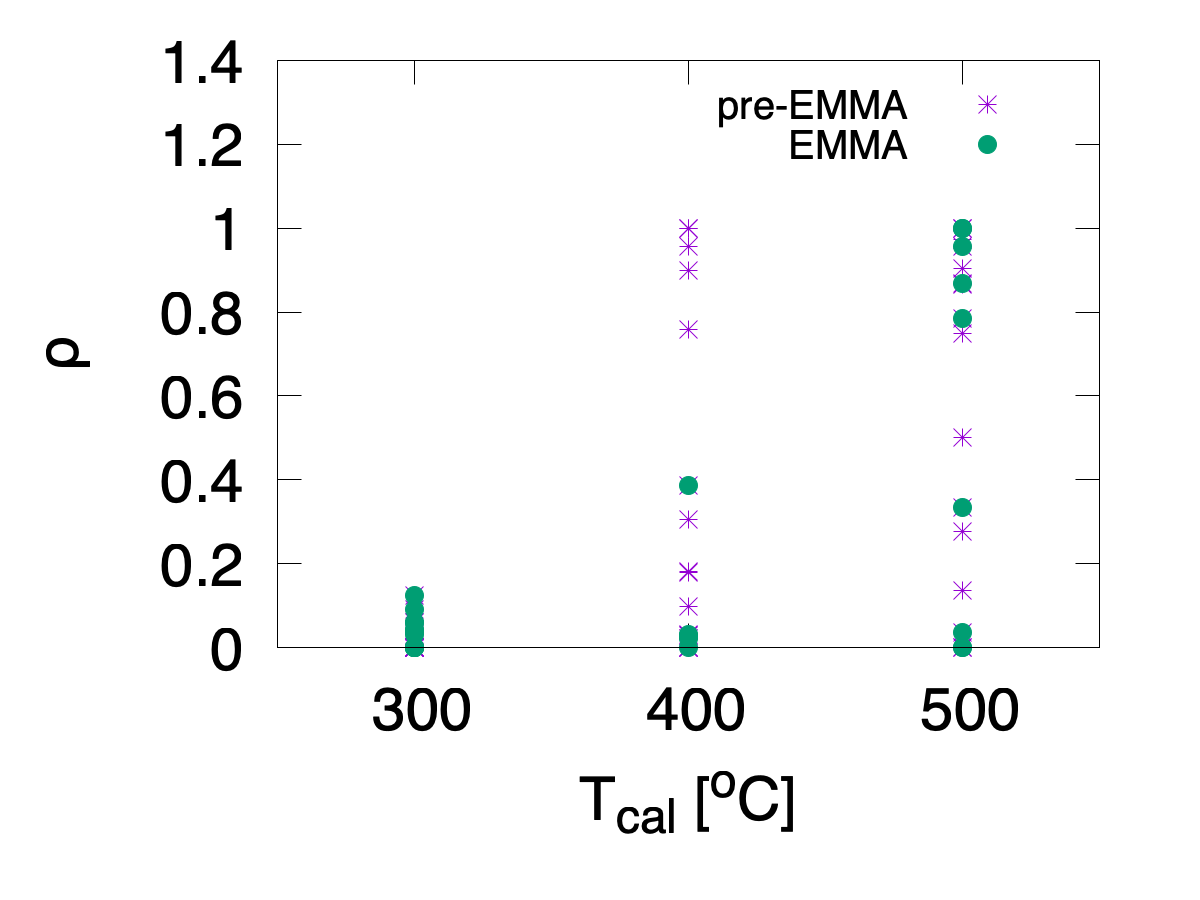
\includegraphics[width=.98\textwidth]{Pics/stats/phd-tcal.png}
        \caption{} \label{fig:phd-tcal}
    \end{subfigure}
	\caption{$\gamma$ (a) and of $\rho$ (b) of each particle and each generation after initial selection process; \td{add caption for c and d.}} 
    \label{fig:emma-gen}
\end{figure}

%%% EQUATION 
%\subsubsection{Equation}
Equations (\ref{eq:emma-phd3})-(\ref{eq:emma-vcal3}) and (\ref{eq:emma-phd4})-(\ref{eq:emma-vcal4}) represent the \gls{rf}s at $t=3$ and $t=4$, respsectively, rounded to 2 significant digits.
%$h(x)$ is the hinge function (also called a rectifier function) of the simple form $h(x) = max(0,x)$. 
The expression $h(\lambda-6)$ translates into layer count only has an influence if larger than 6 
and $h(6-\lambda)$ into layer count influential only if under 6.
%
The first thing to notice is that prediction functions of each generation depend on the same variables. 
%This means that the algorithm must decide on the variables which explain the most variance independent of optimization weights.
This stems from the fact that the algorithm choses a single minimal set of \gls{bf} to predict all dependent variables. 
%
%\td{Knowing this, makes the decision of adding $\lambda$ and $v_{cal}$ as \textit{optimisands} rather unfortunate. %highly questionable. 
%\td{This makes including $\lambda$ and $v_{cal}$ as dependent variables unfortunate decisions with hindsight.}
%As the \gls{mars} algorithm is greedy,
%Different independent variables compete to be used as \gls{bf} in the prediction functions because of the greediness of the \gls{mars} algorithm. 
%}

\begin{align}
%
%    \label{eq:emma-phd1}
%    \hat{\rho}_1 &= -26  + 0.0025 \cdot T_{DB}\cdot T{Cal}  +  0.056 \cdot  h(6-\lambda)\cdot T_{Cal} \\
%    \label{eq:emma-G1}
%    \hat{\gamma}_1 &= -0.52 + 2.3\cdot 10^{-5} \cdot  T_{DB}\cdot T_{Cal} + 0.00080 \cdot h(6-layr)\cdot T_{cal}\\
%    \label{eq:emma-layr1}
%    \hat{\lambda}_1 &= 7.1 + 8.1\cdot 10^{-5} \cdot T_{DB}\cdot T_{cal} -  0.0056 \cdot  h(6-layr)\cdot T_{cal}\\
%    \label{eq:emma-vcal1}
%    \hat{v}_{cal,1} &= 19 - 0.00025 \cdot  T_{DB}\cdot T_{cal} - 0.0055 \cdot  h(6-layr)\cdot T_{cal}\\
%
%    \label{eq:emma-phd2}
%    \hat{\rho}_2 &= 47\\
%    \label{eq:emma-G2}
%    \hat{\gamma}_2 &= 0.23\\
%    \label{eq:emma-layr2}
%    \hat{\lambda}_2 &= 7.3\\
%    \label{eq:emma-vcal2}
%    \hat{v}_{cal,2} &= 10\\
%
    \label{eq:emma-phd3}
    \hat{\rho}_3 &= 0.075  -   0.0014 \cdot  v_{cal}  +    0.18 \cdot  h(6-\lambda)  + 3.9\cdot 10^{-06} \cdot  v_{cal}\cdot T_{cal} \\
    \label{eq:emma-G3}
    \hat{\gamma}_3 &= 43  -   0.097 \cdot  v_{cal}  +     10 \cdot  h(6-\lambda)  + 0.00026 \cdot  v_{cal}\cdot T_{cal} \\
    \label{eq:emma-layr3}
    \hat{\lambda}_3 &= 9.9  - 0.00064 \cdot  v_{cal}  -     2.7 \cdot  h(6-\lambda)  - 1.3\cdot 10^{-06} \cdot  v_{cal}\cdot T_{cal} \\
    \label{eq:emma-vcal3}
    \hat{v}_{cal,3} &= -5.2\cdot 10^{-15}  +   0.016 \cdot  v_{Cal}  + 1.3\cdot 10^{-15} \cdot  h(6-\lambda)  + 3.9\cdot 10^{-21} \cdot  v_{Cal}\cdot T_{cal} \\
%
    \label{eq:emma-phd4}
    \hat{\rho}_4 &=  -0.87 + 0.0047 \cdot  T_{cal} - 0.00036 \cdot  \lambda\cdot T_{cal}  +  0.0024 \cdot  h(\lambda-6)\cdot T_{DB} \\
    \label{eq:emma-G4}
    \hat{\gamma}_4 &=     -19 + 0.28 \cdot  T_{cal}  - 0.022 \cdot  \lambda\cdot T_{cal}  +  0.16 \cdot  h(\lambda-6)\cdot T_{DB} \\
    \label{eq:emma-layr4}
    \hat{\lambda}_4 &=  6.8 - 0.014 \cdot  T_{cal}  + 0.0018 \cdot  \lambda\cdot T_{cal}  + 0.0060 \cdot  h(\lambda-6)\cdot T_{DB} \\
    \label{eq:emma-vcal4}
    \hat{v}_{cal,4} &=  29 - 0.052 \cdot  T_{cal}  + 0.0011 \cdot  \lambda\cdot T_{cal}  -  0.011 \cdot  h(\lambda-6)\cdot T_{DB} 
\end{align}

The coefficients in equations (\ref{eq:emma-phd3}) and (\ref{eq:emma-G3}) have the same signs and differ by a factor of roughly 100.
This fits the data well (see appendix \ref{sec:app-emma}), but the positive influence of the layer count $\lambda$ is counter intuitive 
as one would expect more layers to be more insulating and thus result in lower conductance and a lower probability of holes going all the way trough the \gls{zro} layers. %pin hole density. 
The coefficients of the $v_{cal} \cdot T_{cal}$ interaction in equations (\ref{eq:emma-phd3}) and (\ref{eq:emma-G3}) 
seem low, but - considering the minimum value of the interaction of \num{36000} - have a higher influence on $\rho_3$ and $\gamma_3$ than the $h(6-\lambda)$ term. 
%It's positive the hinge
It is astonishing that the knot of the hinge function for equations (\ref{eq:emma-phd3})-(\ref{eq:emma-vcal3}) was chosen so low; 
basically only including the influence of $\lambda=4$.
Meaning for equations (\ref{eq:emma-phd3}) and (\ref{eq:emma-G3}) that the lowest layer count produces worse samples which is intuitive, but more than 6 layers don't improve the insulation. 
On the positive side, the calcination heating rate $v_{cal}$ (see equation (\ref{eq:emma-vcal3})) has been predicted perfectly within numerical precision. 

%%% T=4
The coefficients of equations (\ref{eq:emma-phd4}) and (\ref{eq:emma-G4}) show the same pattern 
as equations (\ref{eq:emma-phd3}) and (\ref{eq:emma-G3}): identical signs and factor 100. 
The choice of \gls{bf}s in combination with their coefficient signs seems more plausibel
for (\ref{eq:emma-phd4}) and (\ref{eq:emma-G4}) than for (\ref{eq:emma-phd3}) and (\ref{eq:emma-G3}). 
$\lambda$ decreases $\hat{\gamma}$ and $\hat{\rho}$ and additionally the lowest $\lambda$ increases the two \textit{optimisands}. 
% TCAL ON OPTIMIZANDS
The influence of $T_{cal}$ on the measures of conductance ($\rho$ and $\gamma$) is higly interesting. 
It was expected that 
calcination temperatures under \oc{400} do not suffice to produce compact layers and 
that therefore the resulting layer does not insulate as well. 
%\td{xxx}
\textit{Optimsands} $\hat\rho$ and $\hat{\gamma}$ increase with higher calcination temperature 
according to equations \ref{eq:emma-phd4} and \ref{eq:emma-G4}, 
ergo the resistance decreases and the conductance increases with increasing calcination temperature contrary to expectations.
% DESCRIBE COEFFEICIENTS
Furthermore, the influence of the $T_{cal}$ term is the largest of all terms on $\hat{\rho}$ and $\hat{\gamma}$ and also on $\hat\lambda$ and $\hat{v}_{cal}$.
The coefficient of the $\lambda\cdot T_{cal}$ interaction is about a tenth in size of the $T_{cal}$ coefficient, 
but has the extra factor $\lambda$ of up to 12, resulting in the products of coefficients and independent variable being in the same order of magnitude for $T_{cal}$ and $T_{cal}\cdot v_{cal}$.
It can be noted that the coefficient of the $\lambda\cdot T_{cal}$ interaction always has contrary sign to $T_{cal}$ coefficient. 
This negative correlation could hint a compensation of the overestimated influence of $T_{cal}$ on the \textit{optimisands}.
%It should be doubted, though, that the $layr$ only appears as interaction term 
%together with $T_{cal}$ and $T_{DB}$, which seems rather than an artefact. 
%
%It seems rather an artefact of noise that the $\lambda$ only appears as interaction 
%with $T_{cal}$ and $T_{DB}$. 
From the analysis of coefficients it can be said, that the most important factor according to EMMA is $T_{cal}$, followed by $\lambda$, then $T_DB$ and then the rest of the independent variables. 
I highly doubt though that the specific interactions proposed by EMMA are indeed meaningful. 

%%% MSE
For each generation the \gls{mse} was calculated for which only samples 
from the optimisation were used which were available at the time of prediction. 
That means 15 samples for $t=1$ and 30 sampes for $t=4$ were used to calculate respective \gls{mse}s. 
The \gls{mse} is 64, 158, 54 and 50 for $t=1,2,3,4$, respectively. 
It is interesting that although prediction functions for $t=3$ perfectly predicted $v_{cal}$ 
the combined \gls{mse} for $t=4$ is lower. 
The high \gls{mse} at $t=2$ can be explained by the prediction functions being only constant values. 
Apart from the second generation the \gls{mse} decreases  over time, 
which shows that the algorithm works. 
This decrease in \gls{mse} might be attributed to overfitting, though. 
%The \gls{mse} for each generation was also calculated between predicted values for pre-optimisation samples to check for overfitting, 
The \gls{mse} for each generation's prediction function was also calculated with pre-optimisation samples, which are unseen data. 
The error sank again with each generation (except for the second generation): 102, 118, 58, 50, respectively for $t=1,2,3,4$. 
%This shows 
The decrease of \gls{mse} with out-of-sample data shows that the regularization method 
of the \gls{mars} algorithm in principle works on investigated samples. 

%\td{It should be noted, that the validation \gls{mse} for $t=1$ is much higher.}
The high validation \gls{mse} (nearly 1.5 fold instead of circa 1 fold of \gls{mse}) 
for $t=1$ shows the poor prediction ability at the beginning which improved with generations.
This decrease in validation \gls{mse} supports the hypothesis stated at the beginning of this section: 
the measure of conductance was underestimated and improved over time.
%\td{why is \gls{mse} higher with higher values? No homoscedasticity ( equality of variance)?
%Or rather \gls{mse} at $t=2$ high because \gls{rf}s at $t=2$ poor and gen=2 samples are chosen with help of \gls{rf} at $t=2$? 
%}

\td{plot g and p vs TCal, calc avg of p and g for each gen, append pre-emma to appendix}
%%% PROBLEMS 
Even though the main \textit{optimisands} were minimized as required, the \gls{rf}s were not satisfactory. 
The two main problems were too many independent variables and too many dependent variables. 
Both seem closely related and overcomplicate the optimization, but both come with their own implications. 
Too many independent variables make it harder to distinguish variance due to random error (due to unmeasured and uncontrolled variables) from variance due to dependency of chosen dependent varibales. 
This is mainly because of the curse of dimensionality\cite{friedman1988fitting} which makes it hard to collect enough data for each dimension. 
%
In the here presented optimisation model the data points per independent variable 
(events per predictor variable EPV) are as low as 5. 
By eliminating three independent variables the EVP could rise to 10, which is stated 
as rule of tumb for mulitvariate regression\cite{vittinghoff2007relaxing}. 
The results obtained with limited sample number deliver some insightfulness %are quite respectable. 
considering an EPV of 20-50 stated in the original \gls{mars} paper\cite{friedman1991multivariate} 
and an EVP of around 20 in the original \gls{emma} paper\cite{villanova2010function}. 
%In the original \gls{emma} paper\cite{villanova2010function} the EVP is 20.
%\td{In the original \gls{mars} paper\cite{friedman1991multivariate} the model is said 
%to work well on 20-50 events per predictor varibale.
%In the current model EPV are around 5, which is even low for a conservative 
%rule of thumbs of 10-15 EPV\cite{vittinghoff2007relaxing}.
%Not even rule of thumb of 10 EPV \cite{vittinghoff2007relaxing}
%Inspect \cite{friedman1988fitting,friedman1991multivariate} for further \gls{mars} discussion. 
%"The curse-of-dimensionality is fundamental and cannot be directly overcome."- Friedman 1988\cite{friedman1988fitting}.
%}
%
The main problem about too many independent variables specific to this optimisation procedure 
is that the same set of \gls{bf}s will be used to predict all \textit{optimisands}.
This leads to competition between the \gls{bf}s as not all dependent variables may depend on the same independent variables. 
This effect is reinforced by the choice of two independent variables as dependent variables. % (IVDV). 
Independent variables as dependent variables will likely be chosen in \gls{bf}s, 
for including them in the \gls{rf}s is an easy way to reduce the \gls{mse}.
These \gls{bf}s then "take away places" of \gls{bf}s predicting other dependent variables in the \gls{rf}. %\td{(cf. musical chairs)} 
This in turn can lead to wrong predictions and therefore inefficient choice of future samples. 



\td{
%%%%%%%%%%%%%%%%%%%%%%%%%%%%%%%%%%%%%%%%%%%%%%%%%%%%%%%%%%%%%%%%%%%%%%%%%%%%%%%%%%%%%%%%
\subsubsection{rational behind including $v_{cal}$ and $\lambda$ as optimisands}
The heating rate of the calcination process $v_{cal}$ and the number of layers $\lambda$ 
were included as dependent variables with the objective to maximize with a relative weight of 0.05 each.
The idea was to maximize $v_{cal}$ and minimize $\lambda$ in order to minimize the process time. 
Another thought behind including $v_{cal}$ and $\lambda$ was to test if the algorithm would correctly predict those. 
}
%
%Three major flaws behind this consideration became obvious with time: 
%
\
\ds{
(1) The true function for predicting $v_{cal}$ and $\lambda$ are $v_cal*60$ (\oc{}/\h{} instead of \oc{}/\minutes{}) and $\lambda$, respectively. 
The algorithm will tend to include those values into the prediction function for 
all dependent variables and possibly exclude others which have more influence 
on $\gamma$ and $\rho$ (see equations (\ref{eq:emma-G4})? and (\ref{eq:emma-phd4})?).
%
(2) The algorithm would be influenced by those values to choose samples, which potentially optimize $v_{cal}$ and/or $\lambda$ but not $G$ or $\rho$. 
%
(3) needlessly making the problem more complicate %, important time (around 10\% of the samples) could have been replaced with more insightful samples. 
\begin{itemize}
    \item Every output var is independent of each other, so $v_{cal}$ can act as test 
heating rate was one of the dependent variables with the intention of minimizing the variable. 
It can also be used as test to see how well the EMMA performs (or rather, more precisely MARS).
Even if it didn't influence the fit for the other splines, but it influences the choice of samples therefore it might have slowed down the process
Overall there were too many variables involved for such a small dataset
        that means that adding dependent variables influences \td{previous variables}
\end{itemize}
}
\td{look at emma papers}
\td{change G to gamma and write enr to every figure}
\td{in \cite{friedman1991multivariate} the model is said to work well on $\frac{N}{n}$ ratios (aka events per predictor varibale (EPV)) of 20-50. 
EPV is around 5 for this model.
Not even rule of thumb of 10 EPV \cite{vittinghoff2007relaxing}
Inspect \cite{friedman1988fitting,friedman1991multivariate} for further \gls{mars} discussion. 
"The curse-of-dimensionality is fundamental and cannot be directly overcome."- Friedman 1988\cite{friedman1988fitting}.
}




%%%%%%%%%%%%%%%%%%%%%%%%%%%%%%%%%%%%%%%%%%%%%%%%%%%%%%%%%%%%%%%%%%%%%%%%%%%%%%%%%%%%%%%%5
%\subsubsection{how did evolve over time?}


\iffalse
\begin{figure}
\centering
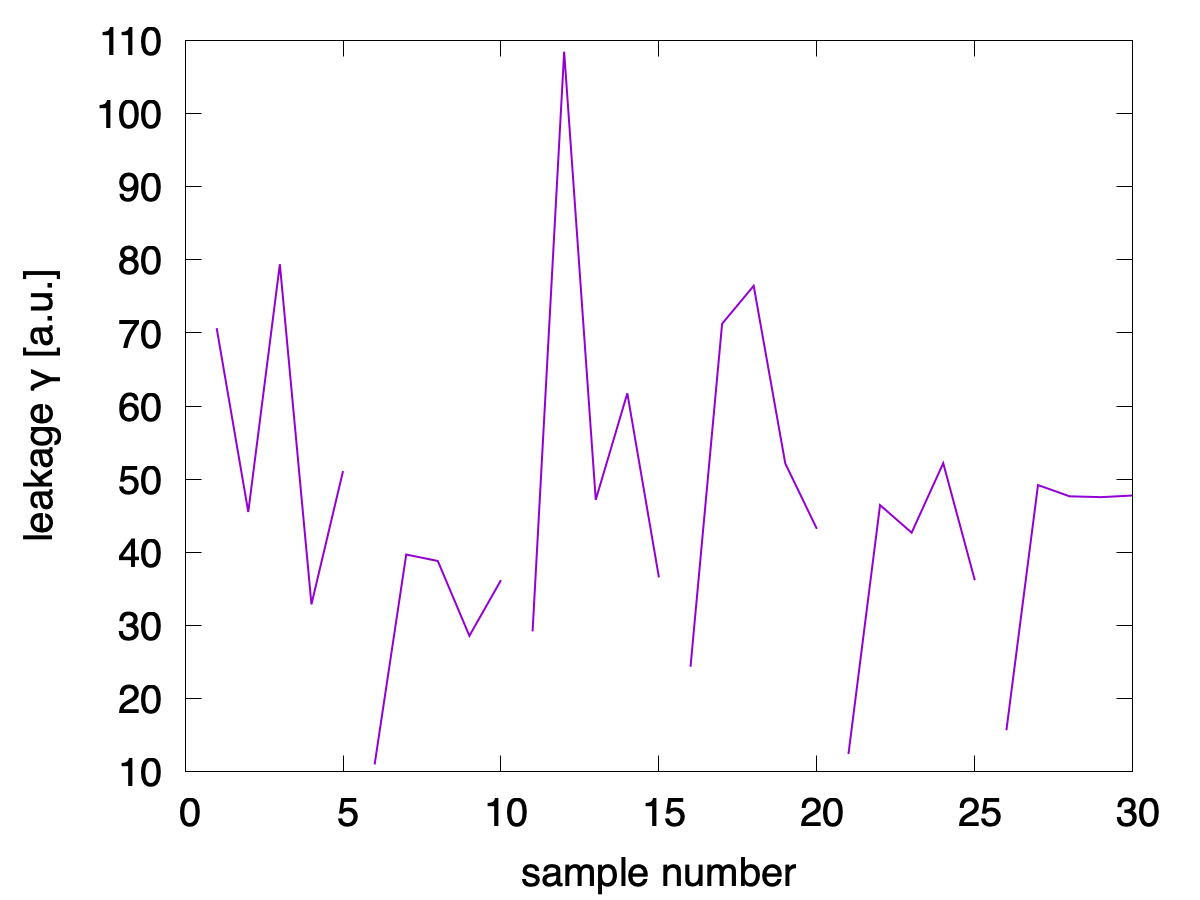
\includegraphics[width=.6\textwidth]{Pics/stats/G-t.png}
    \caption{conductivity G [a.u.] against sample number (is this even correct?)}
    \label{fig:G-t}
\end{figure}

\td{TODO: check if the sorted correctly? Make generation graph with boxplot }
\td{TODO: visualize} how the population moved across the space (with parallel coordinates? or see page 121)
\url{https://stackoverflow.com/questions/30228281/gnuplot-parallel-coordinates-axes-plot-key-annotation}
\fi
